\section{Basic Simulation Parameters}
\label{section:basic}


\subsection{Non-bonded interaction parameters and computations}
\label{section:electdesc}

\NAMD\ has a number of options that control the way that non-bonded
interactions are calculated.  These options are interrelated and
can be quite confusing, so this section attempts to explain the
behavior of the non-bonded interactions and how to use these
parameters.

\subsubsection{Non-bonded van der Waals interactions}
The simplest non-bonded 
interaction is the van der Waals interaction.  In 
\NAMD, van der Waals interactions are always truncated at the 
cutoff distance, specified by {\tt cutoff}.  
The main option that effects van der Waals interactions
is the {\tt switching} parameter.  With this option set to {\tt on},
a smooth switching function will be used to truncate the
van der Waals potential energy smoothly at the cutoff distance.  
A graph of the van der Waals 
potential with this switching function is shown in Figure 
\ref{fig:switching}.  If {\tt switching} is set to {\tt off}, the 
van der Waals energy is just abruptly truncated at the cutoff 
distance, so that energy may not be conserved.  

\begin{figure}[htb]
  \center{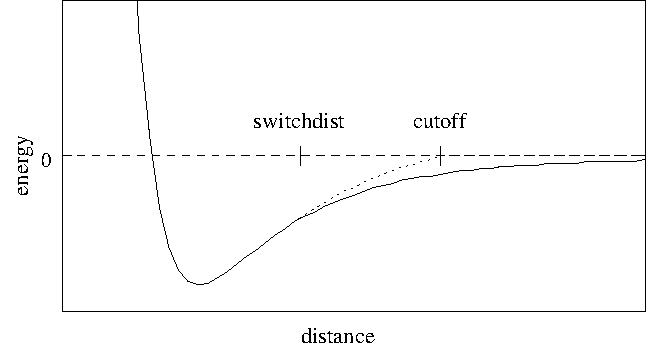
\includegraphics{figures/switching}}
  \caption[Graph of van der Waals potential with and without switching]
  {\small Graph of van der Waals potential with and without the
  application of the switching function.  With the switching function
  active, the potential is smoothly reduced to 0 at the cutoff distance.
  Without the switching function, there is a discontinuity where the
  potential is truncated.}
  \label{fig:switching}
\end{figure}

The switching function used is based on the X-PLOR switching
function.  The parameter {\tt switchdist} specifies the distance
at which the switching function should start taking effect to
bring the van der Waals potential to 0 smoothly at the cutoff distance.  
Thus, the value of {\tt switchdist} must always be less than that 
of {\tt cutoff}.


\subsubsection{Non-bonded electrostatic interactions}
The handling of electrostatics is slightly
more complicated due to the incorporation of multiple timestepping for full
electrostatic interactions.  There are two cases to consider, one where
full electrostatics is employed and the other where electrostatics
are truncated at a given distance.
\prettypar
First let us consider the latter case, where electrostatics are truncated at
the cutoff distance.  Using this scheme, all electrostatic interactions
beyond a specified distance are ignored, or assumed to be zero.  If
{\tt switching} is set to {\tt on}, rather than having a discontinuity
in the potential
at the cutoff distance, a shifting function is applied to the electrostatic
potential as shown in Figure \ref{fig:shifting}.  As this figure shows, the
shifting function shifts the entire potential curve so that the curve
intersects the x-axis at the cutoff distance.  This shifting function
is based on the
shifting function used by X-PLOR.

\begin{figure}[htb]
  \center{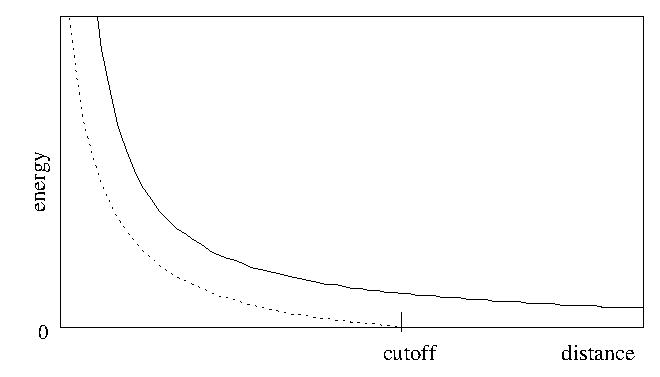
\includegraphics{figures/shifting}}
  \caption[Graph of electrostatic potential with and without shifting function]
  {\small Graph showing an electrostatic potential with and without the
  application of the shifting function.}
  \label{fig:shifting}
\end{figure}

Next, consider the case where full electrostatics are calculated.  In this
case, the electrostatic interactions are not truncated at any distance.  In
this scheme, the {\tt cutoff} parameter has a slightly different meaning
for the electrostatic interactions --- it represents
the {\it local interaction distance\/}, or distance within which electrostatic
pairs will be directly calculated every timestep.  Outside of this distance,
interactions will be calculated only periodically.  These forces
will be applied using a multiple timestep integration scheme as described in
Section \ref{section:fmadesc}.

\begin{figure}[htb]
  \center{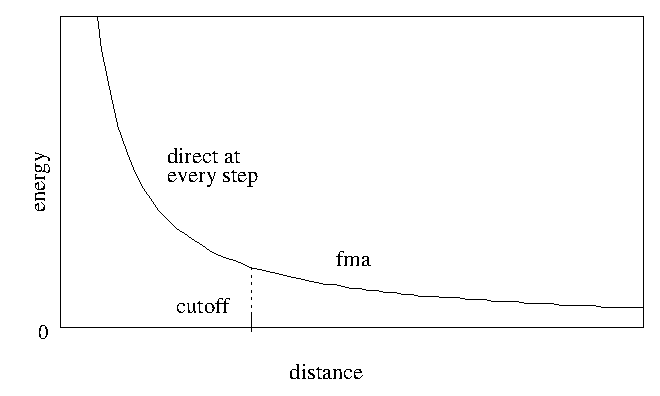
\includegraphics{figures/fmaOn}}
  \caption[Graph of electrostatic split between short and long range forces]
  {\small Graph showing an electrostatic potential 
  when full electrostatics are used within \NAMD, 
  with one curve portion calculated directly 
  and the other calculated using DPMTA.}
  \label{fig:fmaOn}
\end{figure}

\subsubsection{Nonbonded interaction distance-testing}
The last critical parameter for non-bonded
interaction calculations is the parameter {\tt pairlistdist}.  To reduce the
cost of performing the non-bonded interactions, \NAMD\ 1.X used a {\it non-bonded
pair list} which contained all pairs of atoms for which
non-bonded interactions
should be calculated.  Performing the search for pairs of atoms that
should have their interactions calculated is an expensive operation.  Thus,
the pair list is only calculated periodically, once per cycle.   Unfortunately,
pairs of atoms move relative to each other during the steps between preparation
of the pair list.  Because of this, if the pair list were built to include
only
those pairs of atoms that are within the cutoff distance
when the list is generated, it would
be possible 
for atoms to drift closer together
than the cutoff distance during subsequent timesteps and yet not
have their non-bonded interactions calculated.  
\prettypar
Let us consider a concrete example to better understand this.  Assume that the
pairlist is built once every ten timesteps and that the cutoff
distance is 8.0 \AA.  Consider a pair
of atoms A and B that are 8.1 \AA\ apart when the pairlist is built.
If the pair list
includes only those atoms within the cutoff distance, this pair would not
be included in the list.  Now assume that after five timesteps, atoms
A and B have moved to only 7.9 \AA\ apart.  A and B are now within the
cutoff distance of each other, and should have their
non-bonded interactions calculated.
However, because the non-bonded interactions are based solely on the pair list
and the pair list will not be rebuilt for another five timesteps, this pair
will be ignored for five timesteps causing energy not to be conserved 
within the system.  
\prettypar
To avoid this problem, the parameter {\tt pairlistdist} allowed the user
to specify a distance greater than the {\tt cutoff} distance for pairs
to be included in the pair list, as shown in Figure \ref{fig:pairlistdist}.
Pairs that are included in the pair list but are outside the cutoff distance
are simply ignored.  So in the above example, if the {\tt pairlistdist}
were set to $10.0$ \AA, then 
the atom pair A and B would be included in the pair list, even though
the pair would initially be ignored because they are further apart than
the cutoff distance.  As the pair moved closer and entered the cutoff
distance, because the pair was already in the pair list, the non-bonded
interactions would immediately be calculated and energy conservation
would be preserved.  The value of {\tt pairlistdist} should be chosen
such that no atom pair moves more than 
$\mbox{{\tt pairlistdist}}-\mbox{{\tt cutoff}}$ 
in one cycle.  This will insure energy conservation.

\begin{figure}[htb]
  \center{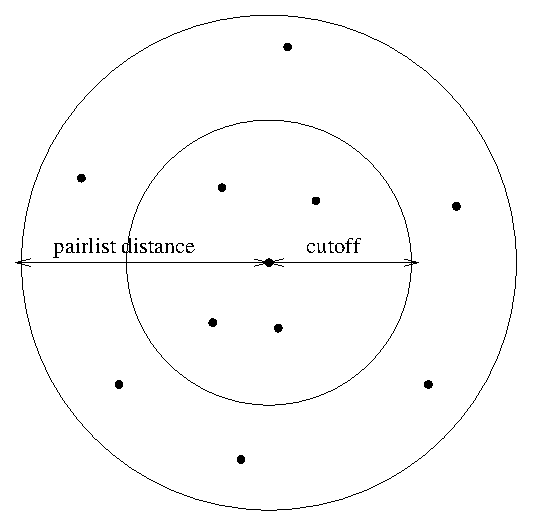
\includegraphics{figures/pairlistdist}}
  \caption[Example of cutoff and pairlist distance uses]
  {{\small Depiction of the difference between the cutoff distance and the
  pair list distance.  The pair list distance specifies a sphere that is
  slightly larger than that of the cutoff so that pairs are allowed to
  move in and out of the cutoff distance without causing energy conservation
  to be disturbed.}}
  \label{fig:pairlistdist}
\end{figure}

NAMD 2.X eliminated the explicit use of pairlists in order to reduce memory usage in light of equally efficient distance-testing algorithms.
Specifically, it was realized that building a pairlist on top of the existing spatial decomposition was only marginally more efficient than actually testing atom distances at every timestep given efficient methods for dealing with nonbonded exclusions.
The {\tt pairlistdist} parameter now serves the same function, but is instead used to determine the minimum patch size.
Unless the {\tt splitPatch} parameter is explicitly set to {\tt position}, hydrogen atoms will be placed on the same patch as the ``mother atom'' to which they are bonded.
These {\em hydrogen groups} are then distance tested against each other using only a cutoff increased by the the value of the {\tt hgroupCutoff} parameter.
The size of the patches is also increased by this amount.
\NAMD\ functions correctly even if a hydrogen atom and its mother atom are separated by more than half of {\tt hgroupCutoff} by breaking that group into its individual atoms for distance testing.
Warning messages are printed if an atom moves outside of a safe zone surrounding the patch to which it is assigned, indicating that {\tt pairlistdist} should be increased in order for forces to be calculated correctly and energy to be conserved.

\subsection{Full electrostatic integration}
\label{section:fmadesc}

To further reduce the cost of computing full electrostatics, 
\NAMD\ uses a multiple timestepping integration scheme.  In this scheme, 
the total force acting on each atom is broken into two pieces, a quickly varying local 
component and a slower long range component.  
The local force component is defined in terms of a {\it splitting function}.  The local force component consists of all bonded and van der Waals interactions
as well as that portion of electrostatic interactions for pairs that are separated by less than the local interaction distance determined by the splitting function.  
The long range component consists only of 
electrostatic interactions outside of the local interaction distance.
Since the long range forces are slowly varying, they are not evaluated
every timestep.  Instead, they are evaluated every $k$ timesteps,
specified by the \NAMD\ parameter {\tt fullElectFrequency}.  
An impulse of $k$ times the long range force is applied to the system
every $k$ timesteps (i.e., the r-RESPA integrator is used).
For appropriate values of $k$,
it is believed that the error introduced by this infrequent evaluation
is modest compared to the error already incurred by the use of the numerical
(Verlet) integrator.  
%The performance of \NAMD\ with the use of DPMTA to provide 
%full electrostatics approximately doubles the 
%run time of a simulation as compared to \NAMD\ with an 
%$8.0$ \AA\ electrostatic cutoff.  
Improved methods for incorporating these long range forces
are currently being investigated, 
with the intention of improving accuracy as well as 
reducing the frequency of long range force evaluations.  
\prettypar
In the scheme described above, the van der Waals forces are still 
truncated at the local interaction distance.  
Thus, the van der Waals cutoff distance 
forms a lower limit to the local interaction distance.  While this is
believed to be sufficient, there are investigations underway to remove
this limitation and provide full van der Waals calculations in 
${\mathcal O}(N)$ time as well.  


\subsection{\NAMD\ configuration parameters}
\label{section:config_basic}

\subsubsection{Timestep parameters}

\begin{itemize}
\item
\NAMDCONF{numsteps}{number of timesteps}{positive integer}
{\label{param:numsteps}
%% This parameter is {\it required\/} for every simulation.
The number of simulation timesteps to be performed.  
An integer greater than 0 is acceptable.  
The total amount of simulation 
time is $\mbox{{\tt numsteps}} \times \mbox{{\tt timestep}}$.}

\item
\NAMDCONFWDEF{timestep}{timestep size (fs)}{non-negative decimal}{1.0}
{The timestep size to use when integrating each step of the simulation.  
The value is specified in femtoseconds.}

\item
\NAMDCONFWDEF{firsttimestep}{starting timestep value}{non-negative integer}{0}
{The number of the first timestep.  This value is typically used only 
when a simulation is a continuation of a previous simulation.  In this 
case, rather than having the timestep restart at 0, a specific timestep 
number can be specified.}

\item
\NAMDCONFWDEF{stepspercycle}{timesteps per cycle}{positive integer}{20}
{Number of timesteps in each cycle.  Each cycle represents the number 
of timesteps between atom reassignments.
For more details on non-bonded force evaluation, see
Section \ref{section:electdesc}.}


\end{itemize}

\subsubsection{Simulation space partitioning}

\begin{itemize}
%\item
%\NAMDCONF{eleccutoff}%
%{local interaction distance for electrostatic calculations (\AA)}%
%{positive decimal}%
%{If DPMTA is active, this distance defines the local interaction length
%for the DPMTA algorithm.
%Otherwise, this value specifies the distance at which
%electrostatic interactions are truncated.
%If {\tt eleccutoff} is defined, it supersedes {\tt cutoff}.
%If {\tt eleccutoff} is not defined, then \verb }cutoff} {\em must}
%be defined.
%See Section \ref{section:electdesc} for a further discussion
%of this configuration value.}

%\item
%\NAMDCONF{vdwcutoff}%
%{local interaction distance for van der Waals calculations (\AA)}%
%{positive decimal}%
%{This value specifies the distance at which
%van der Waals interactions are truncated.
%If {\tt vdwcutoff} is defined, it supersedes {\tt cutoff}.
%If {\tt vdwcutoff} is not defined, then \verb }cutoff} {\em must}
%be defined.
%See Section \ref{section:electdesc} for a further discussion
%of this configuration value.}

\item
\NAMDCONF{cutoff}
{local interaction distance common to both electrostatic 
and van der Waals calculations (\AA)}
{positive decimal}
{%This value can substitute for either {\tt eleccutoff}
%or {\tt vdwcutoff} if either of those is undefined.
See Section \ref{section:electdesc} for more information.}

\item
\NAMDCONFWDEF{switching}{use switching function?}{{\tt on} or {\tt off}}
{{\tt off}}
{If {\tt switching} is
specified to be {\tt off}, then a truncated cutoff is performed.
If {\tt switching} is turned {\tt on}, then smoothing functions
are applied to both the electrostatics and van der Waals forces.
For a complete description of the non-bonded force parameters see
Section \ref{section:electdesc}.  If {\tt switching} is set to
{\tt on}, then {\tt switchdist} must also be defined.}

%\item
%\NAMDCONF{elecswitchdist}{distance at which to activate switching function for %electrostatic calculations (\AA)}{positive decimal $\leq$ {\tt eleccutoff}}
%{Distance at which the switching function
%used to smooth the truncation of
%electrostatic forces should begin to take effect.  
%This parameter only has meaning if {\tt switching} is 
%set to {\tt on}.  
%The value of {\tt elecswitchdist} must be less than
%or equal to the value of {\tt eleccutoff}, since the switching function
%is only applied on the range from {\tt elecswitchdist} to {\tt eleccutoff}.
%If {\tt elecswitchdist} is defined, it supersedes {\tt switchdist}.
%If {\tt elecswitchdist} is not defined and {\tt switching} is
%{\tt on}, then \verb }switchdist} {\em must} be defined.
%For a complete description of the non-bonded force parameters, see
%Section \ref{section:electdesc}.
%}

%\item
%\NAMDCONF{vdwswitchdist}%
%{distance at which to activate switching function 
%for van der Waals calculations (\AA)}%
%{positive decimal $\leq$ {\tt vdwcutoff}}%
%{Distance at which the switching function
%used to smooth the truncation of
%van der Waals forces should begin to take effect.  
%This parameter only has meaning if {\tt switching} is 
%set to {\tt on}.  
%The value of {\tt vdwswitchdist} must be less than
%or equal to the value of {\tt vdwcutoff}, since the switching function
%is only applied on the range from {\tt vdwswitchdist} to {\tt vdwcutoff}.
%If {\tt vdwswitchdist} is defined, it supersedes {\tt switchdist}.
%If {\tt vdwswitchdist} is not defined and {\tt switching} is
%{\tt on}, then \verb }switchdist} {\em must} be defined.
%For a complete description of the non-bonded force parameters, see
%Section \ref{section:electdesc}.
%}

\item
\NAMDCONF{switchdist}
{distance at which to activate switching function 
for electrostatic and van der Waals calculations (\AA)}
{positive decimal $\leq$ {\tt cutoff}}
{Distance at which the switching function
should begin to take effect.  
This parameter only has meaning if {\tt switching} is 
set to {\tt on}.  
The value of {\tt switchdist} must be less than
or equal to the value of {\tt cutoff}, since the switching function
is only applied on the range from {\tt switchdist} to {\tt cutoff}.  
For a complete description of the non-bonded force parameters see
Section \ref{section:electdesc}.}

\item
\NAMDCONFWDEF{pairlistdist}
{distance between pairs for inclusion in pair lists (\AA)}
{positive decimal $\geq$ {\tt cutoff}}
{{\tt cutoff}}
{
A pair list is generated each cycle, 
containing pairs of atoms for which 
electrostatics and van der Waals interactions will be calculated.
This parameter is used when {\tt switching} is set to {\tt on} to
specify the allowable distance between atoms for inclusion in the
pair list.  
This parameter is equivalent to the X-PLOR parameter {\tt CUTNb}.
If no atom moves more than {\tt pairlistdist}$-${\tt cutoff} during
one cycle, then there will be no jump in electrostatic or van der
Waals energies when the next pair list is built.  Since such a jump
is unavoidable when truncation is used, this parameter may only
be specified when {\tt switching} is set to {\tt on}.  If this
parameter is not specified and {\tt switching} is set to {\tt on},
the value of {\tt cutoff} is used.  
A value of at least one greater than {\tt cutoff} is recommended.  
}

\item
\NAMDCONFWDEF{splitPatch}
{how to assign atoms to patches}
{{\tt position} or {\tt hydrogen}}
{{\tt hydrogen}}
{
When set to {\tt hydrogen}, hydrogen atoms are kept on the same patch as their parents, allowing faster distance checking and rigid bonds.
}

\item
\NAMDCONFWDEF{hgroupCutoff (\AA)}
{used for group-based distance testing}
{positive decimal}
{2.5}
{
This should be set to twice the largest distance which will ever occur between a hydrogen atom and its mother.  Warnings will be printed if this is not the case.  This value is also added to the margin.
}

\item
\NAMDCONFWDEF{margin}
{extra length in patch dimension (\AA)}{positive decimal}{0.0}
{An internal tuning parameter used in determining the size of the cubes 
of space with which \NAMD\ uses to partition the system.  The value of 
this parameter will not change the physical results of the simulation.  
Unless you are very motivated to get the {\it very} best 
possible performance, just leave this value at the default.}

%\item
%\NAMDCONFWDEF{plMarginCheck}%
%{perform pairlist margin check?}{{\tt yes} or {\tt no}}{{\tt no}}%
%{\label{param:margincheck}
%If this parameter is activated, a check will be performed during 
%each timestep to detect atoms that may have violated the margin 
%between the {\tt pairlistdist} and {\tt cutoff} distances.  
%Such violations will be output by \NAMD.}

\end{itemize}

\subsubsection{Basic dynamics}

\begin{itemize}
\item
\NAMDCONF{exclude}
{exclusion policy to use}
{{\tt none}, {\tt 1-2}, {\tt 1-3}, {\tt 1-4}, or {\tt scaled1-4}}
{\label{param:exclude}
%% This parameter is {\it required\/} for every simulation.
This parameter specifies which pairs of bonded atoms should
be excluded from non-bonded
interactions.  With the value of {\tt none}, no bonded pairs of atoms 
will be excluded.  With the value of {\tt 1-2}, all atom pairs that
are directly connected via a linear bond will be excluded.  With the
value of {\tt 1-3}, all {\tt 1-2} pairs will be excluded along with
all pairs of atoms that are bonded to a common
third atom (i.e., if atom A is bonded to atom B and atom B is bonded
to atom C, then the atom pair A-C would be excluded).
With the value of {\tt 1-4}, all {\tt 1-3} pairs will be excluded along
with all pairs connected by a set of two bonds (i.e., if atom A is bonded
to atom B, and atom B is bonded to atom C, and atom C is bonded to
atom D, then the atom pair A-D would be excluded).  With the value
of {\tt scaled1-4}, all {\tt 1-3} pairs are excluded and all pairs
that match the {\tt 1-4} criteria are modified.  The electrostatic
interactions for such pairs are modified by the constant factor
defined by {\tt 1-4scaling}.  
The van der Waals interactions are modified
by using the special 1-4 parameters defined in the parameter files.}

\item
\NAMDCONF{temperature}{initial temperature (K)}{positive decimal}
{\label{param:temperature}
Initial temperature value for the system.  
Using this option will generate a random
velocity distribution for the initial velocities 
for all the atoms such that the system 
is at the desired temperature.  
Either the {\tt temperature} 
or the {\tt velocities}/{\tt binvelocities}
option must be defined to determine an initial set of velocities.  
Both options cannot be used together.}

\item
\NAMDCONFWDEF{COMmotion}{allow center of mass motion?}
{{\tt yes} or {\tt no}}{{\tt no}}
{
Specifies whether or not motion of 
the center of mass of the entire system is allowed.  
If this option is set to {\tt no}, the initial velocities of the system 
will be adjusted to remove center of mass motion of the system.
Note that this does not preclude later center-of-mass motion due to 
external forces such as random noise in Langevin dynamics, boundary
potentials, and harmonic restraints.}

\item
\NAMDCONFWDEF{dielectric}{dielectric constant for system}
{decimal $\geq$ 1.0}{1.0}
{Dielectric constant for the system.  A value of 1.0 implies no modification
of the electrostatic interactions.  Any larger value will lessen the
electrostatic forces acting in the system.}

\item
\NAMDCONFWDEF{1-4scaling}{scaling factor for 1-4 interactions}
{0 $\leq$ decimal $\leq$ 1}{1.0}
{Scaling factor for 1-4 interactions.  This factor is only used when the
{\tt exclude} parameter is set to {\tt scaled1-4}.  In this case, this
factor is used to modify the electrostatic interactions between 1-4 atom
pairs.  If the {\tt exclude} parameter is set to anything but 
{\tt scaled1-4}, this parameter has no effect regardless of its value.}

\item
\NAMDCONFWDEF{seed}{random number seed}{positive integer}
{pseudo-random value based on current UNIX clock time}
{Number used to seed the random number generator 
if {\tt temperature} or {\tt langevin} is selected.  This can be
used so that consecutive simulations produce the same results.
If no value is specified, \NAMD\ will choose a pseudo-random
value based on the current UNIX clock time.  The random number
seed will be output during the simulation startup so that
its value is known and can be reused for subsequent simulations.
Note that if Langevin dynamics are used in a parallel simulation 
(i.e., a simulation using more than one processor) 
even using the same seed will {\it not} guarantee reproducible results.
}

\item
\NAMDCONFWDEF{rigidBonds}{controls if and how ShakeH is used}{{\tt none},
{\tt water}, {\tt all}}{{\tt none}} 
{When {\tt rigidBonds} is {\tt all}, the bond between each hydrogen
and its mother atom is fixed to the nominal bond length given in the
parameter file.  When {\tt water} is selected, only the bonds between
the hydrogens and the oxygen in water molecules are constrained.  
For the default case {\tt none}, no lengths are constrained.
}

\item
\NAMDCONFWDEF{rigidTolerance}{allowable bond-length error for ShakeH (\AA)}
{positive decimal}{0.00001}
{
The ShakeH algorithm is assumed to have converged when all constrained
bonds differ from the nominal bond length by less than this amount.
}

\item
\NAMDCONFWDEF{rigidIterations}{maximum ShakeH iterations}{positive integer}{100}
{
The maximum number of iterations ShakeH will perform before giving up
on constraining the bond lengths.  If the bond lengths do not
converge, a warning message is printed, and the atoms are left at the
final value achieved by ShakeH.  
Although the default value is 100, 
convergence is usually reached after fewer than 10 iterations.
}

\end{itemize}

\subsubsection{DPMTA parameters}

{\em DPMTA is no longer included in the released NAMD binaries.
We recommend that you instead use PME with a periodic system because
it conserves energy better, is more efficient, and is better parallelized.
If you must have the fast multipole algorithm you may compile \NAMD\ yourself.} 

These parameters control the options to DPMTA, an algorithm
used to provide full electrostatic interactions.  DPMTA is a
modified version of the FMA (Fast Multipole Algorithm) and, 
unfortunately, most of the parameters still refer to FMA
rather than DPMTA for historical reasons.  Don't be confused!
\prettypar
For a further description of how exactly full electrostatics
are incorporated into \NAMD, see Section \ref{section:fmadesc}.
For a greater level of detail about DPMTA and the specific
meaning of its options, see the DPMTA distribution which is
available via anonymous FTP from the site {\tt ftp.ee.duke.edu}
in the directory {\tt /pub/SciComp/src}.

\begin{itemize}

\item
\NAMDCONFWDEF{FMA}{use full electrostatics?}{{\tt on} or {\tt off}}{{\tt off}}
{Specifies whether or not 
the DPMTA algorithm from Duke University should be used 
to compute the full electrostatic interactions.  If set to 
{\tt on}, DPMTA will be used with a multiple timestep integration scheme 
to provide full electrostatic interactions as detailed in Section 
\ref{section:fmadesc}.  {\em DPMTA is no longer included in released binaries.}}

\item
\NAMDCONFWDEF{FMALevels}{number of levels to use in multipole expansion}{positive integer}{5}
{Number of levels to use for the multipole expansion.  This parameter
is only used if {\tt FMA} is set to {\tt on}.  
A value of 4 should be sufficient for systems with less than 10,000 atoms.  
A value of 5 or greater should be used for larger systems. }

\item
\NAMDCONFWDEF{FMAMp}{number of multipole terms to use for FMA}{positive integer}{8}
{Number of terms to use in the multipole expansion.  
This parameter is only used if {\tt FMA} is set to {\tt on}.  
If the {\tt FMAFFT} is set to {\tt on}, then this value must 
be a multiple of 4.  The default value of 8 should be suitable
for most applications.}

\item
\NAMDCONFWDEF{FMAFFT}{use DPMTA FFT enhancement?}{{\tt on} or {\tt off}}{{\tt on}}
{Specifies whether or not the DPMTA code should use the FFT enhancement 
feature.  This parameter is only used if {\tt FMA} is set to {\tt on}.  
If {\tt FMAFFT} is set to {\tt on}, the value of {\tt FMAMp} must be 
set to a multiple of 4.  
This feature offers substantial benefits only for values 
of {\tt FMAMp} of 8 or greater.  This feature will substantially 
increase the amount of memory used by DPMTA.}

%%  REMOVE THIS AS A DOCUMENTED FEATURE.  WE USE stepspercycle INSTEAD.  
%%
%%  \item
%%  \NAMDCONF{FMAfrequency}{number of timesteps between DPMTA calculations}{positive integer}
%%  {This parameter specifies the number of timesteps between each
%%  invocation of the DPMTA algorithm.}

\item
\NAMDCONFWDEF{FMAtheta}{DPMTA theta parameter (radians)}{decimal}{0.715}
{This parameter specifies the value of the theta parameter
used in the DPMTA calculation.  The default value is based on
recommendations by the developers of the code.}

\item
\NAMDCONFWDEF{FMAFFTBlock}{blocking factor for FMA FFT}{positive integer}{4}
{The blocking factor for the FFT enhancement to DPMTA.
This parameter is only used if both {\tt FMA} and {\tt FMAFFT} 
are set to {\tt on}.  The default value of 4 should be suitable
for most applications.}

\end{itemize}

\subsubsection{PME parameters}

PME stands for Particle Mesh Ewald and is an efficient
full electrostatics method for use with periodic boundary conditions.
None of the parameters should affect energy conservation, although they may affect the accuracy of the results and momentum conservation.

\begin{itemize}

\item
\NAMDCONFWDEF{PME}{Use particle mesh Ewald for electrostatics?}{{\tt yes} or {\tt no}}{{\tt no}}
{Turns on particle mesh Ewald.}

\item
\NAMDCONFWDEF{PMETolerance}{PME direct space tolerance}{positive decimal}{$10^{-6}$}
{Affects the value of the Ewald coefficient and the overall accuracy of the results.}

\item
\NAMDCONFWDEF{PMEInterpOrder}{PME interpolation order}{positive integer}{4 (cubic)}
{Charges are interpolated onto the grid and forces are interpolated off using this many points, equal to the order of the interpolation function plus one.}

\item
\NAMDCONF{PMEGridSizeX}{number of grid points in x dimension}{positive integer}
{The grid size partially determines the accuracy and efficiency of PME.
For speed, {\tt PMEGridSizeX} should have only small integer factors (2, 3 and 5).}

\item
\NAMDCONF{PMEGridSizeY}{number of grid points in y dimension}{positive integer}
{The grid size partially determines the accuracy and efficiency of PME.
For speed, {\tt PMEGridSizeY} should have only small integer factors (2, 3 and 5).}

\item
\NAMDCONF{PMEGridSizeZ}{number of grid points in z dimension}{positive integer}
{The grid size partially determines the accuracy and efficiency of PME.
For speed, {\tt PMEGridSizeZ} should have only small integer factors (2, 3 and 5).}

\item
\NAMDCONFWDEF{PMEProcessors}{processors for FFT and reciprocal sum}{positive integer}{larger of x and y grid sizes up to all available processors}
{For best performance on some systems and machines, it may be necessary to
restrict the amount of parallelism used.  Experiment with this parameter if
your parallel performance is poor when PME is used.}

\item
\NAMDCONFWDEF{FFTWEstimate}{Use estimates to optimize FFT?}{{\tt yes} or {\tt no}}{{\tt no}}
{Do not optimize FFT based on measurements, but on FFTW rules of thumb.
This reduces startup time, but may affect performance.}

\item
\NAMDCONFWDEF{FFTWUseWisdom}{Use FFTW wisdom archive file?}{{\tt yes} or {\tt no}}{{\tt yes}}
{Try to reduce startup time when possible by reading FFTW ``wisdom'' from a file, and saving wisdom generated by performance measurements to the same file for future use.
This will reduce startup time when running the same size PME grid on the same number of processors as a previous run using the same file.}

\item
\NAMDCONFWDEF{FFTWWisdomFile}{name of file for FFTW wisdom archive}{file name}{FFTW\_NAMD\_{\em version}\_{\em platform}.txt}
{File where FFTW wisdom is read and saved.
If you only run on one platform this may be useful to reduce startup times for all runs.
The default is likely sufficient, as it is version and platform specific.}

\item
\NAMDCONFWDEF{useDPME}{Use old DPME code?}{{\tt yes} or {\tt no}}{{\tt no}}
{Switches to old DPME implementation of particle mesh Ewald.
The new code is faster and allows non-orthogonal cells so you
probably just want to leave this option turned off.  If you set
{\tt cellOrigin} to something other than $(0,0,0)$ the energy may differ
slightly between the old and new implementations.
{\em DPME is no longer included in released binaries.}
}

\end{itemize}

\subsubsection{Full direct parameters}

The direct computation of electrostatics 
is not intended to be used during 
real calculations, but rather as a testing or 
comparison measure.  Because of the ${\mathcal O}(N^2)$ 
computational complexity for performing 
direct calculations, this is {\it much} 
slower than using DPMTA or PME to compute full 
electrostatics for large systems.
In the case of periodic boundary conditions,
the nearest image convention is used rather than a
full Ewald sum.

\begin{itemize}

\item
\NAMDCONFWDEF{FullDirect}{calculate full electrostatics directly?}{{\tt yes} or {\tt no}}{{\tt no}}
{Specifies whether or not direct computation of 
full electrostatics should be performed.}

\end{itemize}

\subsubsection{Multiple timestep parameters}

One of the areas of current research being studied using \NAMD\ is the
exploration of better methods for performing multiple timestep integration.
Currently the only available method is the impulse-based Verlet-I or r-RESPA
method which is stable for timesteps up to 4~fs for long-range electrostatic
forces, 2~fs for short-range nonbonded forces, and 1~fs for bonded forces
Setting {\tt rigid all} (i.e., using SHAKE) increases these timesteps to
6~fs, 2~fs, and 2~fs respectively but eliminates bond motion for hydrogen.
The mollified impulse method (MOLLY) reduces the resonance which limits
the timesteps and thus increases these timesteps to 6~fs, 2~fs, and 1~fs
while retaining all bond motion.

\begin{itemize}

\item
\NAMDCONFWDEF{fullElectFrequency}{number of timesteps between full electrostatic evaluations}{positive integer factor of {\tt stepspercycle}}{{\tt nonbondedFreq}}
{This parameter specifies the number of timesteps between each full electrostatics evaluation.
It is recommended that {\tt fullElectFrequency} be chosen so that 
the product of {\tt fullElectFrequency} and {\tt timestep} does 
not exceed $4.0$ unless {\tt rigidBonds all} or {\tt molly on} is specified, 
in which case the upper limit is perhaps doubled.}

\item
\NAMDCONFWDEF{nonbondedFreq}{timesteps between nonbonded evaluation}{positive integer factor of {\tt fullElectFrequency}}{1}
{This parameter specifies how often short-range nonbonded interactions should be calculated.  Setting {\tt nonbondedFreq} between 1 and {\tt fullElectFrequency} allows triple timestepping where, for example, one could evaluate bonded forces every 1 fs, short-range nonbonded forces every 2 fs, and long-range electrostatics every 4 fs.} 

\item
\NAMDCONFWDEF{MTSAlgorithm}{MTS algorithm to be used}{{\tt impulse/verletI} or {\tt constant/naive}}{{\tt impulse}}
{Specifies the multiple timestep algorithm used to integrate the 
long and short range forces.  {\tt impulse/verletI} is the same as r-RESPA.
{\tt constant/naive} is the stale force extrapolation method.}


\item
\NAMDCONFWDEF{longSplitting}{how should long and short range forces be split?}{{\tt xplor}, {\tt c1}}{{\tt c1}}
{Specifies the method used to split electrostatic forces between long 
and short range potentials.  
The {\tt xplor} option uses the X-PLOR shifting function, 
and the {\tt c1} splitting uses 
the following $C^1$ continuous shifting 
function \mycite{Humphreys \ETAL}{HUMP94}:  
\begin{list}{}{}
\item
$SW(r_{ij}) = 0$ if $|{{\vec{r}}_{ij}}| > R_{\mathit off}$
\item
$SW(r_{ij}) = 1$ if $|{{\vec{r}}_{ij}}| \leq R_{\mathit on}$
\item
% $SW(r_{ij}) = \frac{ {\left({R_{\mathit off}}^2 - {r_{ij}}^2\right)}^2
% \left({R_{\mathit off}}^2 + 2{r_{ij}}^2 - 3{R_{\mathit on}}^2\right)}
% {{\left({R_{\mathit off}}^2 - {R_{\mathit on}}^2\right)}^3}$
if $R_{\mathit off} > |{{\vec{r}}_{ij}}| \geq R_{\mathit on}$
\end{list}
}
where
\begin{list}{}{}
\item
$R_{\mathit on}$ is a constant defined using the configuration value 
{\tt switchdist} 
\item
$R_{\mathit off}$ is specified using the configuration value {\tt cutoff}
\end{list}

\item
\NAMDCONFWDEF{molly}{use mollified impulse method (MOLLY)?}
{{\tt on} or {\tt off}}{{\tt off}}
{
This method eliminates the components of the long range electrostatic
forces which contribute to resonance along bonds to hydrogen atoms,
allowing a fullElectFrequency of 6 (vs.\ 4) with a 1~fs timestep
without using {\tt rigidBonds all}.  You may use {\tt rigidBonds water} but
using {\tt rigidBonds all} with MOLLY makes no sense since the degrees of
freedom which MOLLY protects from resonance are already frozen.
}

\item
\NAMDCONFWDEF{mollyTolerance}{allowable error for MOLLY}
{positive decimal}{0.00001}
{
Convergence criterion for MOLLY algorithm.
}

\item
\NAMDCONFWDEF{mollyIterations}{maximum MOLLY iterations}{positive integer}{100}
{
Maximum number of iterations for MOLLY algorithm.
}

\end{itemize}

